\chapter{Ergebnisse}

Sofern nicht anders erwähnt, beziehen sich die Laufzeiten auf Systeme mit zwei Intel Xeon Gold 6230 Prozessoren mit einer Taktrate von 2.1 Ghz und 180GB RAM.
Die Ergebnisse wurden auf gleichen System, aber nicht auf demselben erzeugt.

\section{Untersuchung der Graphen}

Der Fokus dieser Arbeit liegt auf drei Sichtbarkeitsgraphen, welche jeweils einen Ausschnitt des Globus beinhalten.
Für jeden dieser drei Graphen existiert zusätzlich eine Triangulierung, deren kürzeste Pfade eine untere Schranke zu Sichtbarkeitsgraphen darstellt
\autoref{table:input_graphs} listet die Graphen auf.
Die Graphen mit dem Präfix \emph{aegaeis} beinhalten das Ägäische Meer, mit \emph{medi} das Mittelmeer und mit \emph{pata} die Chilenische Fjorde.
Graphen mit dem Postfix \emph{visibility} sind Sichtbarkeitsgraphen, mit \emph{graph} Triangulierungen.
Die bearbeiteten Graphen sind ungerichtet, werden im folgenden jedoch als gerichtet betrachtet.
Insbesondere ist die in \autoref{table:input_graphs} aufgelistete Anzahl an Kanten gerichtetet zu interpretieren,
die ungerichtete Kante $\{a, b\}$ wird also doppelt gezählt als $(a, b)$ und $(b, a)$.

\begin{table}[h!]
  \centering
  \begin{tabular}{
      l % Graph
      S[table-format = 7.0] % Zeit
      S[table-format = 9.0] % Zeit
      S[table-format = 4.1] % Zeit
    }
    \toprule
    {Graph}            & {\# Knoten} & {\# Kanten} & {$\varnothing$ Grad} \\ \midrule
    aegaeis-graph      & 524881      & 2795322     & 5.32562999994        \\
    aegaeis-visibility & 201040      & 310231834   & 1543.13486868        \\
    medi-graph         & 795606      & 4223566     & 5.30861506826        \\
    medi-visibility    & 310114      & 730772544   & 2356.46421638        \\
    pata-graph         & 2240339     & 11632900    & 5.1924731034         \\
    pata-visibility    & 1002171     & 315653758   & 314.969958221        \\ \bottomrule
  \end{tabular}
  \caption{Bearbeite Graphen}
  \label{table:input_graphs}
\end{table}

\subsection{Dijkstra}

Für die Berechnung des Speedups der in dieser Arbeit verwendeten Methoden wurden für jeden Graphen \num{1000} sequentielle $s$-$t$-Dijkstra-Suchen ausgeführt und die durchschnittliche Laufzeit ermittelt.
Die ermittelten Zeiten für das Finden und Erstellen des kürzesten Pfades sind in Tabelle \ref{fig:ergebnisse:dijkstra} dargestellt.
Aus den Ergebnissen geht hervor, dass die Sichtbarkeitsgraphen im Vergleich zu ihren Triangulierungen deutlich höhere Laufzeiten aufweisen.

Zusätzlich zur durchschnittlichen Laufzeit wurde die die Durchschnittswerte der Hop-Länge, des Dijsktra-Rank und der Queue pops über \num{10000} $s$-$t$-Dijkstra-Suchen ermittelt, um ein Verständnis für die Laufzeiten zu erlangen.
Dabei zeigte sich, dass die durchschnittliche Hop-Länge in den Sichtbarkeitsgraphen signifikant kürzer ist als in den Triangulierungen.
Trotz der geringeren Anzahl an Knoten in den Sichtbarkeitsgraphen ist die durchschnittliche Anzahl an Queue Pops jedoch höher.
Dies deutet darauf hin, dass der Einsatz einer Warteschlange mit einer \emph{Decrease-Key}-Funktion die Effizienz der Dijkstra-Suche potenziell verbessern könnte.
Der Versuch, die Suchzeit durch die Verwendung einer solchen Warteschlange zu reduzieren, schlug jedoch fehl.

\begin{table}[h!]
  \centering
  \begin{tabular}{
      l % Graph
      S[table-format = 4.1] % Zeit
      S[table-format = 3.0] % hop-länge
      S[table-format = 7.0] % rank
      S[table-format = 7.0] % queue pops
    }
    \toprule
    {Graph}            & {$\varnothing$ $t({spd})$} & {$\varnothing$  Hop-Länge} & {$\varnothing$ Dijkstra Rank} & {$\varnothing$ Queue pops} \\
                       & {(\si{\ms})}               &                            &                               &                            \\
    \midrule
    aegaeis-graph      & 60.281198                  & 215.7201                   & 260447.36                     & 325845.56                  \\
    aegaeis-visibility & 630.434928                 & 16.311                     & 98650.82                      & 517346.63                  \\
    medi-graph         & 87.08376                   & 340.445                    & 394855.78                     & 494553.97                  \\
    medi-visibility    & 1279.67479                 & 23.6149                    & 154092.42                     & 959206.4                   \\
    pata-graph         & 265.825771                 & 883.979                    & 1120841.9                     & 1387047.8                  \\
    pata-visibility    & 1017.695977                & 63.817                     & 498570.2                      & 2429689.8                  \\ \bottomrule
  \end{tabular}
  \caption{Durschnitliche Kennwerte der Dijkstra Suchen (über \num{10000} Suchen)}
  \label{fig:ergebnisse:dijkstra}
\end{table}

\subsection{Knotengrade}

Weiter wurde die Verteilung der Knotengrade untersucht, die enstanden Histogramme sind in \autoref{ergebnisse:fig:degree_hist} erstellt.
In allen untersuchten Sichtbarkeitsgraphen haben mindestens 90\% der Knoten einen Grad von weniger als \num{2000}.

\begin{figure}[p]
  \begin{subfigure}[b]{0.5\textwidth}
    \resizebox{\textwidth}{!}{%
      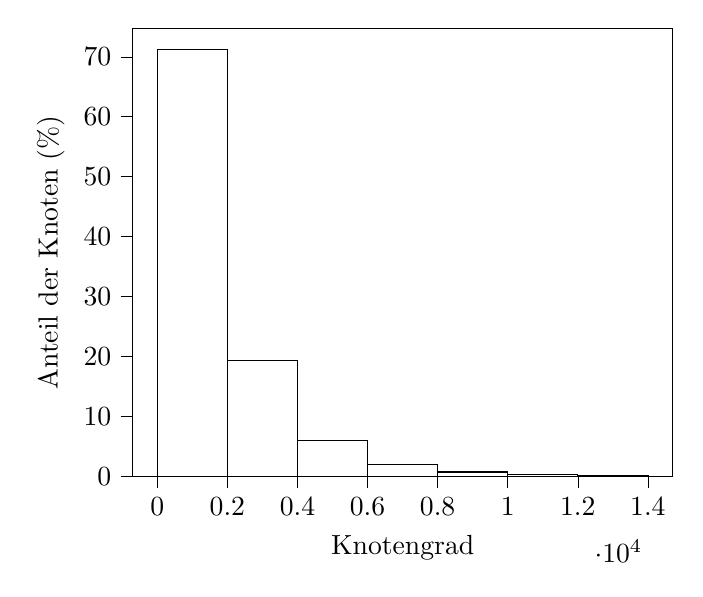
\begin{tikzpicture}
        \begin{axis}[
            tick align=outside,
            tick pos=left,
            xmin=-698, xmax=14702,
            xtick style={color=black},
            xtick distance=2000,
            ymin=0, ymax=0.747618384401001,
            ytick style={color=black},
            ytick={0,0.1,0.2,0.3,0.4,0.5,0.6,0.7,0.8},
            yticklabels={0,10,20,30,40,50,60,70,80},
            xlabel={Knotengrad},
            ylabel={Anteil der Knoten (\%)}
          ]
          \draw[] (axis cs:2,0) rectangle (axis cs:2002,0.712017508953334);
          \draw[] (axis cs:2002,0) rectangle (axis cs:4002,0.194220055711032);
          \draw[] (axis cs:4002,0) rectangle (axis cs:6002,0.0606247512935969);
          \draw[] (axis cs:6002,0) rectangle (axis cs:8002,0.0205382013530728);
          \draw[] (axis cs:8002,0) rectangle (axis cs:10002,0.00766514126545947);
          \draw[] (axis cs:10002,0) rectangle (axis cs:12002,0.00397930760049903);
          \draw[] (axis cs:12002,0) rectangle (axis cs:14002,0.000955033824119655);
        \end{axis}
      \end{tikzpicture}
    }
    \caption{aegaeis-vis}
  \end{subfigure}%
  \begin{subfigure}[b]{0.5\textwidth}
    \resizebox{\textwidth}{!}{%
      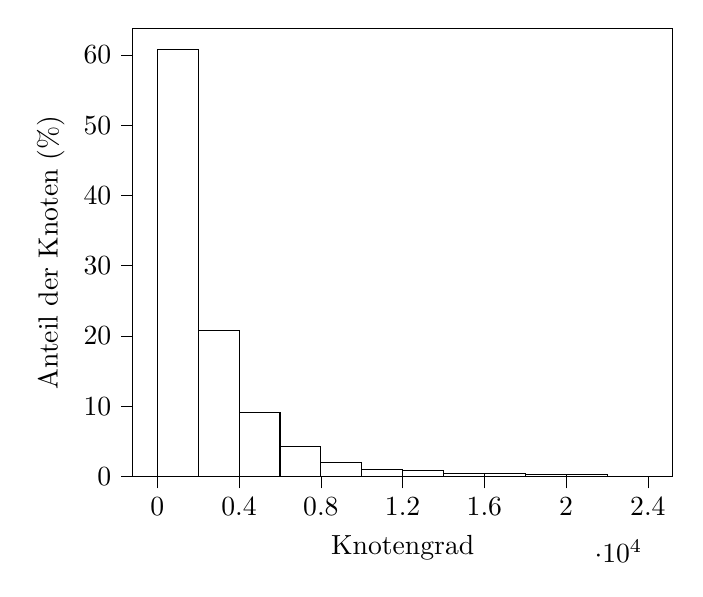
\begin{tikzpicture}
        \begin{axis}[
            tick align=outside,
            tick pos=left,
            xlabel={Knotengrad},
            xmin=-1198, xmax=25202,
            xtick distance=4000,
            xtick style={color=black},
            ylabel={Anteil der Knoten (\%)},
            ymin=0, ymax=0.637890337808629,
            ytick style={color=black},
            ytick={0,0.1,0.2,0.3,0.4,0.5,0.6,0.7},
            yticklabels={0,10,20,30,40,50,60,70}
          ]
          \draw[] (axis cs:2,0) rectangle (axis cs:2002,0.60751460743679);
          \draw[] (axis cs:2002,0) rectangle (axis cs:4002,0.207212784893063);
          \draw[] (axis cs:4002,0) rectangle (axis cs:6002,0.0905080679486225);
          \draw[] (axis cs:6002,0) rectangle (axis cs:8002,0.0423164235317719);
          \draw[] (axis cs:8002,0) rectangle (axis cs:10002,0.0196700589456533);
          \draw[] (axis cs:10002,0) rectangle (axis cs:12002,0.0103219440467273);
          \draw[] (axis cs:12002,0) rectangle (axis cs:14002,0.00818403436132265);
          \draw[] (axis cs:14002,0) rectangle (axis cs:16002,0.00425647177184629);
          \draw[] (axis cs:16002,0) rectangle (axis cs:18002,0.00420165357478464);
          \draw[] (axis cs:18002,0) rectangle (axis cs:20002,0.00342452501643997);
          \draw[] (axis cs:20002,0) rectangle (axis cs:22002,0.00236363167330556);
          \draw[] (axis cs:22002,0) rectangle (axis cs:24002,2.57967986172503e-05);
        \end{axis}
      \end{tikzpicture}
    }
    \caption{medi-vis}
  \end{subfigure}
  \par\bigskip
  \begin{subfigure}[b]{0.5\textwidth}
    \resizebox{\textwidth}{!}{%
      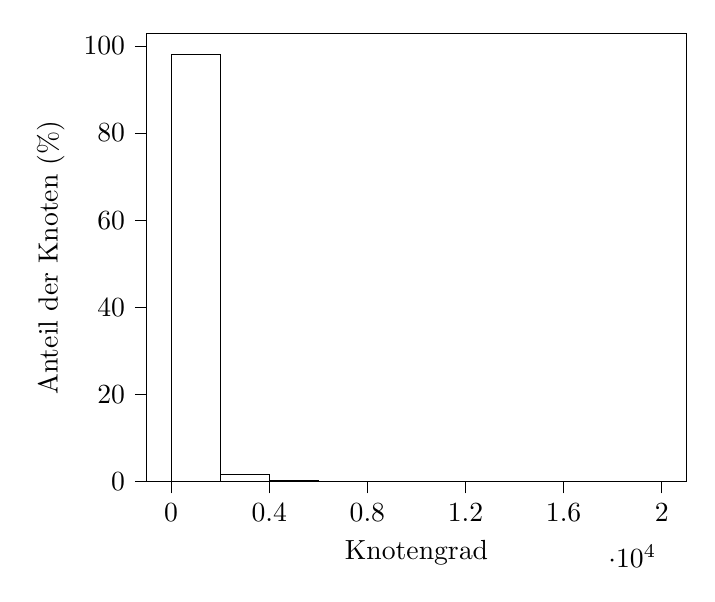
\begin{tikzpicture}
        \begin{axis}[
            tick align=outside,
            tick pos=left,
            xlabel={Knotengrad},
            ylabel={Anteil der Knoten (\%)},
            xmin=-998, xmax=21002,
            xtick style={color=black},
            y grid style={darkgray176},
            xtick distance=4000,
            ymin=0, ymax=1.02857224104146,
            ytick style={color=black},
            ytick={0,0.2,0.4,0.6,0.8,1,1.2},
            yticklabels={0,20,40,60,80,100,120}
          ]
          \draw[] (axis cs:2,0) rectangle (axis cs:2002,0.979592610515676);
          \draw[] (axis cs:2002,0) rectangle (axis cs:4002,0.0169022235303201);
          \draw[] (axis cs:4002,0) rectangle (axis cs:6002,0.00222602483448042);
          \draw[] (axis cs:6002,0) rectangle (axis cs:8002,0.000968834654540784);
          \draw[] (axis cs:8002,0) rectangle (axis cs:10002,0.000297335455255565);
          \draw[] (axis cs:10002,0) rectangle (axis cs:12002,3.99107993631631e-06);
          \draw[] (axis cs:12002,0) rectangle (axis cs:14002,0);
          \draw[] (axis cs:14002,0) rectangle (axis cs:16002,9.97769984079078e-07);
          \draw[] (axis cs:16002,0) rectangle (axis cs:18002,3.99107993642733e-06);
          \draw[] (axis cs:18002,0) rectangle (axis cs:20002,3.99107993631631e-06);
        \end{axis}

      \end{tikzpicture}
    }
    \caption{pata-vis}
  \end{subfigure}
  \caption{Verteilung der Kantengrade}
  \label{ergebnisse:fig:degree_hist}
\end{figure}

Als Indikator dafür, wie sehr sich die Graphen kontrahieren lassen, wurde die Summe der quadratischen Knotengrade berechnet, diese ist in \autoref{table:sum_quad_degree} aufgelistet.
Diese ist bei den Sichtbarkeitsgraphen jeweils um mehrere Größenordnungen größer als bei ihren Triangulierungen.

\begin{table}[ht]
  \centering
  \begin{tabular}{
      l % Graph
      S[table-format = 13.0] % Zeit
    }
    \toprule
    {Graph}            & {$\sum_{v \in V} (\text{Grad}(v))^2$} \\
    \midrule
    aegaeis-graph      & 16024918                              \\
    aegaeis-visibility & 1153579966074                         \\
    medi-graph         & 24163472                              \\
    medi-visibility    & 4667069733248                         \\
    pata-graph         & 65662096                              \\
    pata-visibility    & 426189267238                          \\
    \bottomrule
  \end{tabular}
  \caption{Summe quadratische Knotengrade}
  \label{table:sum_quad_degree}
\end{table}

\section{Graphen-Kontraktion}

Der Ausgangspunkt der Analyse, ob die in dieser Arbeit behandelten Sichtbarkeitsgraphen kontrahiert werden können, war die Anwendung der klassischen Graphen-Kontraktion mit Dijkstra-Suchen.
Dabei kam ein speziell für diese Arbeit entwickeltes Programm zum Einsatz.
Die Reihenfolge der Kontraktionen wurde durch die Kanten-Differenz mit Lazy-Popping bestimmt.

Während es für die triangulierten Graphen möglich war, einen Contracted-Graph zu erstellen, wurde diese Erstellung bei den Sichtbarkeitsgraphen nach drei Tagen abgebrochen, da in dieser Zeit noch nicht einmal alle initialen Kanten-Differenzen berechnet werden konnten.
Die Ergebnisse für die triangulierten Graphen sind in Tabelle \autoref{fig:ergebnisse:ch_graph_kontraktion_triangulierungen} dargestellt.

\begin{table}[h!]
  \centering
  \begin{tabular}{
      l % Graph
      r % Erstellung
      S[table-format = 1.2] % Abkürzungen/Katen
      S[table-format = 9.0] % average time spd
      S[table-format = 4.0] % speedup
    }
    \toprule
    {Graph}       & {Erstellung} & {$\frac{\text{Abkürzungen} (C)}{\text{Kanten} (G)}$} & {$\varnothing$ $t({spd})$} & {Speedup}                          \\
    {}            & {}           & {}                                                   & {(\si{\us})}               & {}                                 \\
    \midrule
    aegaeis-graph & 2m 22s       & \fpeval{3047836/2795322}                             & 313.966                    & \fpeval{(60.281198*1000)/313.966}  \\
    medi-graph    & 3m 17s       & \fpeval{4535136/4223566}                             & 304.089                    & \fpeval{(87.08376*1000)/304.089}   \\
    pata-graph    & 9m 54s       & \fpeval{14187336/11632900}                           & 435.552                    & \fpeval{(265.825771*1000)/435.552} \\  \bottomrule
  \end{tabular}
  \caption{CH Graphen-Kontraktion}
  \label{fig:ergebnisse:ch_graph_kontraktion_triangulierungen}
\end{table}

Bassierend auf den Contracted-Graphen der Triangulierungen wurde jeweils ein Hub-Graph durch Merging erstellt.
Die Ergebnisse hierfür sind in \autoref{fig:ergebnisse:hl_graph_kontraktion_triangulierungen} aufgelistet.

\begin{table}[h!]
  \centering
  \begin{tabular}{
      l % Graph
      r % Erstellung
      S[table-format = 3.0] % label
      S[table-format = 3.2] % average time spd
      S[table-format = 6.] % speedup
    }
    \toprule
    {Graph}       & {Erstellung}     & {$\varnothing$ $\abs{\text{Label}}$} & {$\varnothing$ $t({spd})$} & {Speedup}                        \\
    {}            & {}               & {}                                   & {(\si{\us})}               & {}                               \\
    \midrule
    aegaeis-graph & 7m 11s           & 141.4722365640974                    & 2.334                      & \fpeval{(60.281198*1000)/2.334}  \\
    medi-graph    & 9m \phantom{0}1s & 115.88322360565405                   & 1.893                      & \fpeval{(87.08376*1000)/1.893}   \\
    pata-graph    & 29m 45s          & 133.48887779929734                   & 2.415                      & \fpeval{(265.825771*1000)/2.415} \\
    \bottomrule
  \end{tabular}
  \caption{HL Graphen-Kontraktion}
  \label{fig:ergebnisse:hl_graph_kontraktion_triangulierungen}
\end{table}

Als zusätzlicher Referenzpunkt zur Beurteilung der Qualität der erzeugten Contracted-Graphen sowie der dafür benötigten Zeit wurde ein externes Programm verwendet, um ebenfalls Contracted-Graphen zu erstellen\todo{cite?}.
Die Ergebnisse hierfür sind in \autoref{fig:ergebnisse:fmi_ch_graph_kontraktion_triangulierungen} aufgelistet.

Da dieses Programm ein anderes Speicherformat verwendet, konnten die Anfragezeiten nicht ermittelt werden.
Es wurden jedoch im Vergleich zu dem in dieser Arbeit verwendeten Programm mehr Abkürzungen eingefügt.
Das Programm kontrahiert mehrere Knoten gleichzeitig, indem es \emph{unabhängige Teilmengen} von Knoten identifiziert, was eine effizientere parallele Verarbeitung ermöglicht.\todo{cite!}
Aufgrund des hohen Grades der Sichtbarkeitsgraphen ist jedoch davon auszugehen, dass nur wenige und kleine unabhängige Teilmengen existieren.
Auch dieses Programm lieferte nach drei Tagen Laufzeit auf den Sichtbarkeitsgraphen keine Ergebnisse.

\begin{table}[h!]
  \centering
  \begin{tabular}{
      l % Graph
      r % Erstellung
      S[table-format = 1.2] % Abkürzungen/Katen
      S[table-format = 9.0] % average time spd
      S[table-format = 4.0] % speedup
    }
    \toprule
    {Graph}       & {Erstellung} & {$\frac{\text{Abkürzungen} (C)}{\text{Kanten} (G)}$} \\
    {}            & {(min)}      & {}                                                   \\
    \midrule
    aegaeis-graph & 22s          & \fpeval{(5446922-(2795322/2))/2795322}               \\
    medi-graph    & 34s          & \fpeval{(8156314-(4223566/2))/4223566}               \\
    pata-graph    & 1m 48s       & \fpeval{(23557322-(11632900/2))/11632900}            \\  \bottomrule
  \end{tabular}
  \caption{FMI CH Graphen-Kontraktion}
  \label{fig:ergebnisse:fmi_ch_graph_kontraktion_triangulierungen}
\end{table}

\subsection{Kontraktion mit oberer Schranke}

Die kürzesten Pfaddistanzen in triangulierten Graphen stellen, wie in \autoref{chapter:kontraktion} beschrieben, eine obere Schranke für die Distanzen zwischen Knotenpaaren in den Sichtbarkeitsgraphen dar.
Um den Fehler dieser Schranke zu quantifizieren, wurden die kürzesten Pfaddistanzen von \num{1000000} $s$-$t$-Paaren in den Sichtbarkeitsgraphen analysiert.
Der dabei ermittelte durchschnittliche Fehler pro Hop-Länge ist in \autoref{img:ergebnisse:upper_bound} als Datenreihe $\triangle$ dargestellt.

Diese Abbildung zeigt auch den durchschnittlichen Fehler, der durch den Einsatz von $n$ Hubs entsteht, welche mithilfe eines Hitting-Sets bestimmt wurden.
Zusätzlich wurde der Fehler visualisiert, der sich aus der Wahl der kleinsten oberen Schranke zwischen 80 Hubs und den triangulierten Graphen ergibt.

\begin{figure}[p]% Die Daten in den .csv Dateien sind gelippt auf 100. pgf hat Probleme mit zu großen Zahlen.
  \begin{subfigure}[b]{0.5\textwidth}
    \resizebox{\textwidth}{!}{%
      \begin{tikzpicture}
        \begin{axis}[
            ymax=6,
            xlabel={Hop-Länge},
            ylabel={Fehler (\%)},
            legend style={at={(1,0.475)},anchor=east, nodes={scale=0.8, transform shape}}
          ]
          \addplot+[mark repeat=9] table [x=hops, y=simple_graph_upper_bound, col sep=comma] {data/bounds/aegaeis.csv};
          \addlegendentry{$\triangle$};

          \addplot+[mark repeat=9] table [x=hops, y=10, col sep=comma] {data/bounds/aegaeis.csv};
          \addlegendentry{10 Hubs};

          \addplot+[mark repeat=9] table [x=hops, y=20, col sep=comma] {data/bounds/aegaeis.csv};
          \addlegendentry{20 Hubs};

          \addplot+[mark repeat=9] table [x=hops, y=40, col sep=comma] {data/bounds/aegaeis.csv};
          \addlegendentry{40 Hubs};

          \addplot+[mark repeat=9] table [x=hops, y=80, col sep=comma] {data/bounds/aegaeis.csv};
          \addlegendentry{80 Hubs};

          \addplot+[mark repeat=9] table [x=hops, y=min_80_simple, col sep=comma] {data/bounds/aegaeis.csv};
          \addlegendentry{$\triangle$, 80 Hubs};
        \end{axis}
      \end{tikzpicture}
    }
    \caption{aegaeis-vis}
  \end{subfigure}%
  \begin{subfigure}[b]{0.5\textwidth}
    \resizebox{\textwidth}{!}{%
      \begin{tikzpicture}
        \begin{axis}[
            ymax=6,
            xlabel={Hop-Länge},
            ylabel={Fehler (\%)},
            legend style={at={(1,0.475)},anchor=east, nodes={scale=0.8, transform shape}}
          ]
          \addplot+[mark repeat=12] table [x=hops, y=simple_graph_upper_bound, col sep=comma] {data/bounds/medi.csv};
          \addlegendentry{$\triangle$};

          \addplot+[mark repeat=12] table [x=hops, y=10, col sep=comma] {data/bounds/medi.csv};
          \addlegendentry{10 Hubs};

          \addplot+[mark repeat=12] table [x=hops, y=20, col sep=comma] {data/bounds/medi.csv};
          \addlegendentry{20 Hubs};

          \addplot+[mark repeat=12] table [x=hops, y=40, col sep=comma] {data/bounds/medi.csv};
          \addlegendentry{40 Hubs};

          \addplot+[mark repeat=12] table [x=hops, y=80, col sep=comma] {data/bounds/medi.csv};
          \addlegendentry{80 Hubs};

          \addplot+[mark repeat=12] table [x=hops, y=min_80_simple, col sep=comma] {data/bounds/medi.csv};
          \addlegendentry{$\triangle$, 80 Hubs};
        \end{axis}
      \end{tikzpicture}
    }
    \caption{medi-vis}
  \end{subfigure}
  \par\bigskip
  \begin{subfigure}[b]{0.5\textwidth}
    \resizebox{\textwidth}{!}{%
      \begin{tikzpicture}
        \begin{axis}[
            ymax=6,
            xlabel={Hop-Länge},
            ylabel={Fehler (\%)},
            legend style={at={(1,0.475)},anchor=east, nodes={scale=0.8, transform shape}}
          ]
          \addplot+[mark repeat=25] table [x=hops, y=simple_graph_upper_bound, col sep=comma] {data/bounds/pata.csv};
          \addlegendentry{$\triangle$};

          \addplot+[mark repeat=25] table [x=hops, y=10, col sep=comma] {data/bounds/pata.csv};
          \addlegendentry{10 Hubs};

          \addplot+[mark repeat=25] table [x=hops, y=20, col sep=comma] {data/bounds/pata.csv};
          \addlegendentry{20 Hubs};

          \addplot+[mark repeat=25] table [x=hops, y=40, col sep=comma] {data/bounds/pata.csv};
          \addlegendentry{40 Hubs};

          \addplot+[mark repeat=25] table [x=hops, y=80, col sep=comma] {data/bounds/pata.csv};
          \addlegendentry{80 Hubs};

          \addplot+[mark repeat=25] table [x=hops, y=min_80_simple, col sep=comma] {data/bounds/pata.csv};
          \addlegendentry{$\triangle$, 80 Hubs};
        \end{axis}
      \end{tikzpicture}
    }
    \caption{pata}
  \end{subfigure}
  \caption{Fehler der oberen Schranken}
  \label{img:ergebnisse:upper_bound}
\end{figure}

\todo{Wie performant ist das?}

\section{PEOPLE}

Die in \autoref{chapter:peopel} vorgestellte Methode zur Berechnung von Contracted- und Hub-Graphen lies sich auf die Sichtbarkeitsgraphen und ihre Triangulierungen anwenden.
Hierbei konnten die Hub-Graphen entweder direkt durch PEOPLE zereugt werden oder indem zuerst ein Contracted-Graph erstellt wurde.
Die vertex-to-level-Funktion wurde hierbei jeweils durch ein Hitting-Set über \num{100000} Dijkstra-Pfade ermittelt.
Der Größe der dem Hitting-Set zugrunde liegenden Menge an Pfaden wurde hierbei bewusst relativ klein gewählt, mit der überelgung, dass wenn dies erfolgreich ist, in einem zweiten Schritt mit den erzeugten Hub-Graphen deutlich mehr Pfade erzeugt werden können.

\subsection{Contracted-Graph}

Durch die Berechnung aller ausgehenden Kanten pro Knoten im Downward- und Upward-Graphen konnte sowohl für die Sichtbarkeitsgraphen als auch für deren Triangulierungen jeweils ein Contracted-Graph erstellt werden.
Die Kennzahlen der Erzeug und Anfragezeiten sind in \autoref{table:ergebnisse:people_ch_speedup} aufgeführt.

\begin{table}[h!]
  \centering
  \begin{tabular}{
      l % Graph
      r % S[table-format = 4.0] % Erstellung
      S[table-format = 1.2] % Abkürzungen/Katen
      S[table-format = 3.2] % average time spd
      S[table-format = 3.2] % speedup
    }
    \toprule
    {Graph}            & {Erstellung} & {$\frac{\text{Abkürzungen} (C)}{\text{Kanten} (G)}$} & {$\varnothing$ $t({spd})$} & {Speedup}                       \\
    {}                 & {}           & {}                                                   & {(\si{\ms})}               & {}                              \\ \midrule
    aegaeis-graph      & 20m          & \fpeval{12443056/2795322}                            & 2.290886                   & \fpeval{60.281198/2.290886}     \\
    aegaeis-visibility & 5h 53m       & \fpeval{214987558/310231834}                         & 408.948758                 & \fpeval{630.434928/408.948758}  \\
    medi-graph         & 38m          & \fpeval{20003908/4223566}                            & 3.38788                    & \fpeval{87.08376/3.38788}       \\
    medi-visibility    & 20h 52m      & \fpeval{468641256/730772544}                         & 832.555567                 & \fpeval{1279.67479/832.555567}  \\
    pata-graph         & 5h 42m       & \fpeval{70624466/11632900}                           & 10.16729                   & \fpeval{265.825771/10.16729}    \\
    pata-visibility    & 1d 20h 45m   & \fpeval{613324174/315653758}                         & 288.514849                 & \fpeval{1017.695977/288.514849} \\  \bottomrule
  \end{tabular}
  \caption{Kennwerte von mit PEOPLE erzeugten Contracted-Graphen}
  \label{table:ergebnisse:people_ch_speedup}
\end{table}

Der Speedup der auf diese Weise erzeugten Contracted-Graphen der Triangulierungen ist etwa um eine Größenordnung geringer als der der durch Kontraktion erstellten Contracted-Graphen.
Zudem wurden jweils mehr als dreimal so viele Abkürzungen hinzugefügt.

Auf den Sichtbarkeitsgraphen von aegaeis und medi wurde ein Speedup von nur \num{1.5} erzielt, auf pata von immerhin \num{3.5}.
Im Vergleich zu der Rechenzeit, welche in die Erstellung investiert wurde, ist dies jedoch recht wenig.

\subsection{Hub Graph}

Aus den berechneten Contracted-Graphen konnte durch Merging Hub-Graphen erzeugt werden, wobei zu klären war, ob es schneller ist, zuerst einen Contracted-Graphen und dann einen Hub-Graphen zu erstellen, oder ob es schneller ist, direkt einen Hub-Graphen zu erstellen.

\subsubsection{Merging}

Ein zunächst verwendetes Programm, welches einen Hub-Graph aus einem Contracted-Graphen ohne Parallelisierung erzeugte, war nicht in der Lage, innerhalb von drei Tagen die Hub-Graphen der Sichtbarkeitsgraphen zu erzeugen.
Der Grund hierfür liegt in der schieren Anzahl an Labels und Einträgen, die dabei gemerged werden müssen:
Ein Knoten der Contracted-Graphen der Sichtbarkeitsgraphen hat einen drei- bis vierstelligen Grad, und für jeden dieser Nachbarn gibt es ein Label, das ebenfalls gemerged werden muss
Die Verwendung eines parallelen \emph{reduce}-Algorithmus zum Mergen der Labels eines Knotens führte zu den Ergebnissen in \autoref{table:ergebnisse:hl_ch_bruteforce}.

\begin{table}[h!]
  \centering
  \begin{tabular}{ %MERGING
      l % Graph
      r % Erstellung
      S[table-format = 4.1] % label
      S[table-format = 2.2] % average time spd
      S[table-format = 6.0] % speedup
      S[table-format = 3.1] % average time sp
    }
    \toprule
    {Graph}            & {Erstellung}      & {$\varnothing$ $\abs{\text{Label}}$} & {$\varnothing$ $t({spd})$} & {Speedup$({spd})$}                 & {$\varnothing$ $t({sp})$} \\
    {}                 & {}                & {}                                   & {(\si{\us})}               & {}                                 & {(\si{\us})}              \\
    \midrule
    aegaeis-graph      & 12m               & 225.21998319619112                   & 1.617                      & \fpeval{(60.281198*1000)/1.617}    & 54.266                    \\
    aegaeis-visibility & 7h 35m            & 2447.866444488659                    & 9.382                      & \fpeval{(630.434928*1000)/9.382}   & 17.026                    \\
    medi-graph         & 19m               & 262.34248736183486                   & 1.777                      & \fpeval{(87.08376*1000)/1.777}     & 80.017                    \\
    medi-visibility    & 22h 18m           & 3528.6126965393596                   & 14.887                     & \fpeval{(1279.67479*1000)/14.887}  & 25.867                    \\
    pata-graph         & 1h 22m            & 451.8001829187458                    & 2.526                      & \fpeval{(265.825771*1000)/2.526}   & 264.981                   \\
    pata-visibility    & 14h \phantom{0}7m & 1823.062327697596                    & 16.862                     & \fpeval{(1017.695977*1000)/16.862} & 26.942                    \\
    \bottomrule
  \end{tabular}
  \caption{Kennwerte von mit Merging erstellter Hub-Graphen. Die zugrundeliegenden Contracted-Graphen wurden mit PEOPLE erzeugt.}
  \label{table:ergebnisse:hl_ch_bruteforce}
\end{table}


\subsubsection{PEOPLE}

Die Hub-Graphen wurden ebenfalls durch PEOPLE berechnet.
Die Werte sind in \autoref{table:ergebnisse:hl_bruteforce} zu sehen.
Die Durchschnittliche Label Größe ist minimal anders.

\begin{table}[h!]
  \centering
  \begin{tabular}{ %MERGING
      l % Graph
      r % Erstellung
      S[table-format = 4.1] % label
      S[table-format = 2.2] % average time spd
      S[table-format = 6.] % speedup
      S[table-format = 3.1] % average time sp
    }
    \toprule
    {Graph}            & {Erstellung}         & {$\varnothing$ $\abs{\text{Label}}$} & {$\varnothing$ $t({spd})$} & {Speedup$({spd})$}                 & {$\varnothing$ $t({spd})$} \\
    {}                 & {}                   & {}                                   & {(\si{\us})}               & {}                                 & {(\si{\us})}               \\
    \midrule
    aegaeis-graph      & 1h 26m               & 225.18963155458096                   & 1.612                      & \fpeval{(60.281198*1000)/1.612}    & 53.997                     \\
    aegaeis-visibility & 5h 57m               & 2446.9511241543973                   & 9.595                      & \fpeval{(630.434928*1000)/9.595}   & 17.31                      \\
    medi-graph         & 3h 11m               & 262.32183266591755                   & 1.787                      & \fpeval{(87.08376*1000)/1.787}     & 81.234                     \\
    medi-visibility    & 21h 57m              & 3527.5645951837378                   & 13.506                     & \fpeval{(1279.67479*1000)/13.506}  & 26.671                     \\
    pata-graph         & 1d \phantom{0}4h 26m & 451.71017734369667                   & 2.512                      & \fpeval{(265.825771*1000)/2.512}   & 263.59                     \\
    pata-visibility    & 1d 20h 17m           & 1822.0561604813242                   & 16.635                     & \fpeval{(1017.695977*1000)/16.635} & 27.324                     \\
    \bottomrule
  \end{tabular}
  \caption{Kennwerte von mit PEOPLE erstellen Hub-Graphen}
  \label{table:ergebnisse:hl_bruteforce}
\end{table}

Das Anwenden des des Algorithmus zur Berechnung des Hub GRaphens hat gut funktioniert.


\subsubsection{Vergleich}


Da die Hub-Graphen auf zwei Wegen erzeugt werden können, muss geklärt werden, welcher Weg effizienter ist.
Dazu wurde die Zeit, die für die Erstellung des Contracted-Graphen benötigt wurde, mit der Zeit zum Mergen addiert und anschließend mit der Zeit zur direkten Erstellung eines Hub-Graphen mittels PEOPLE verglichen.
Die entsprechenden Zahlen sind in Tabelle \autoref{table:ergebnisse:vergleich_was_schneller} aufgeführt.

Interessanterweise ist es bei den Sichtbarkeitsgraphen schneller, direkt einen Hub-Graphen zu berechnen, während es bei den triangulierten Graphen effizienter ist, den Umweg über die Contracted-Graphen zu nehmen.

\todo{DIE LABELS SIND MINIMAL UNTERSCHIEDLICH GROß}


\begin{table}[h!]
  \centering
  \begin{tabular}{ %VERGLEICH
      l % Graph
      r
      r
    }
    \toprule
    {Graph}            & {Contracted-Graph \& Merging} & {Hub-Graph}                    \\
    \midrule
    aegaeis-graph      & 32m                           & \bfseries 1h 26m               \\
    aegaeis-visibility & \bfseries 13h 28m             & 5h 57m                         \\
    medi-graph         & 57 m                          & \bfseries 3h 11m               \\
    medi-visibility    & \bfseries 1d 19h 10m          & 21h 57m                        \\
    pata-graph         & 7h \phantom{0} 4m             & \bfseries 1d \phantom{0}4h 26m \\
    pata-visibility    & \bfseries 2d 10h 52m          & 1d 20h 17m                     \\  \bottomrule
  \end{tabular}
  \caption{HL  merged}
  \label{table:ergebnisse:vergleich_was_schneller}
\end{table}

\subsection{Performance Overhead}
Die Erzeugung der ausgehenden Kanten im Contracted-Graph sowie der Label im Hub-Graph erfolgen durch modifizierte Dijkstra-Suchen, beinhaltet aber zusätzlich unter anderem auch die Sammlung von Abkürzungen.

Zur Quantifizierung des zusätzlichen Rechenaufwands wurden für jeden Graphen, für jeweils \emph{10000} Knoten, jeweils zwei Dijkstra Suchen zu alle anderen Knoten durchgeführt.
Die dafür benötigte Rechenzeit wurde anschließend auf die Anzahl der Knoten im Graph skaliert.
\autoref{table:ergebnisse:dijkstra_vs_ch_vs_hl} zeigt die erforderliche Zeit zur Erstellung eines Contracted- und eines Hub-Graphen im Verhältnis zu dieser skalierten Zeit.
Es fällt auf, dass die für die Konstruktion eines Contracted-Graphen benötigte Zeit nur geringfügig kürzer ist als die eines Hub-Graphen.
Dies lässt darauf schließen, dass in den meisten Fällen spät abgebrochen wurde.


\begin{table}[h!]
  \centering
  \begin{tabular}{ %VERGLEICH
      l % Graph
      r % Graph
      S[table-format = 1.3] % average time
      S[table-format = 1.3] % average time
    }
    \toprule
    {Graph}            & {Dijkstra} & {$\frac{\text{Contracted-Graph}}{\text{Dijkstra}}$} & {$\frac{\text{Hub-Graph}}{\text{Dijkstra}}$}   \\ \midrule
    aegaeis-graph      & 46m        & \fpeval{(20)/(46)}                                  & \fpeval{(1*60+26)/(46)}                        \\
    aegaeis-visibility & 5h 19m     & \fpeval{(5*60+53)/(5*60+19)}                        & \fpeval{(5*60+57)/(5*60+19)}                   \\
    medi-graph         & 1h 46m     & \fpeval{(38)/(1*60+46)}                             & \fpeval{(3*60+11)/(1*60+46)}                   \\
    medi-visibility    & 19h 51m    & \fpeval{(20*60+52)/(19*60+51)}                      & \fpeval{(21*60+57)/(19*60+51)}                 \\
    pata-graph         & 14h 55m    & \fpeval{(5*60+42)/(14*60+55)}                       & \fpeval{(1*24*60+4*60+26)/(14*60+55)}          \\
    pata-visibility    & 1d 12h 32m & \fpeval{(1*24*60+20*60+45)/(1*24*60+12*60+32)}      & \fpeval{(1*24*60+20*60+17)/(1*24*60+12*60+32)} \\  \bottomrule
  \end{tabular}
  \caption{todo dijkstra vs ch bruteforce vs hl bruteforce}
  \label{table:ergebnisse:dijkstra_vs_ch_vs_hl}
\end{table}

Für die Triangulierung von Sichtbarkeitsgraphen ist es deutlich effizienter, Contracted-Graphen zu erstellen, anstatt für jeden Knoten zwei vollständige Dijkstra-Suchen durchzuführen und noch effizienter, als einen Hub-Graphen zu erstellen.
Daher ist davon auszugehen, dass die Dijkstra-Suchen häufiger vorzeitig abgebrochen worden konnten.

Um dieses Verhalten besser zu verstehen, wurde die Suche nach ausgehenden Kanten eines Knotens im aeagaeis-Sichtbarkeitsgraphen näher untersucht.
\autoref{fig:ergebnisse:ch_people_suchbaum} zeigt einen entsprechenden Suchbaum.
In der Abbildung repräsentieren schwarze Punkte die Knoten, die als Köpfe für die aus dem weißen Punkt ausgehenden Upward-Kanten fungieren.
Die dünnen Kanten führen zu Knoten, die zum Zeitpunkt ihrer Expansion nicht mehr lebendig waren, die gestrichelten Kanten gehen zu Knoten, die zwar gesehen, aber nicht mehr expandiert wurden.
Für den betrachteten Knoten wurde lediglich ein Bruchteil der insgesamt \num{524881} möglichen Knoten besucht, was die Effizienz dieses Ansatzes unterstreicht.

\begin{figure}[h!]
  \centering
  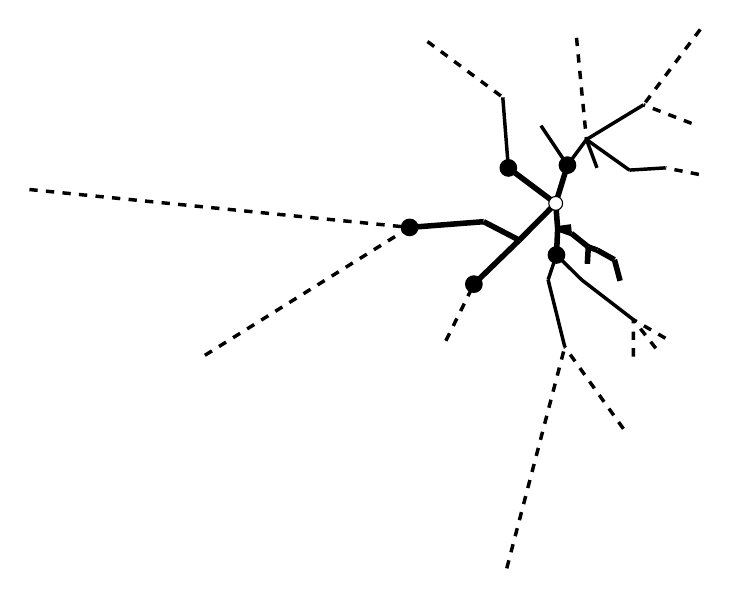
\begin{tikzpicture}[scale=1.5]
    \draw[line width=2] (4.456048319873318, 3.0900255391060227) edge (4.456048319873318, 3.0900255391060227);
    \draw[line width=2] (4.472612660101305, 2.8750437520344008) edge (4.456048319873318, 3.0900255391060227);
    \draw[line width=2] (4.587260603652865, 2.8905717642487616) edge (4.472612660101305, 2.8750437520344008);
    \draw[line width=2] (4.5889971877098645, 2.835738571829438) edge (4.472612660101305, 2.8750437520344008);
    \draw[line width=2] (4.555467757087328, 3.413754167559091) edge (4.456048319873318, 3.0900255391060227);
    \draw[line width=2] (4.46260040552211, 2.6534343050634845) edge (4.472612660101305, 2.8750437520344008);
    \draw[line width=2] (4.1474929335649335, 2.778701673953776) edge (4.456048319873318, 3.0900255391060227);
    \draw[line width=2] (4.05516128339265, 3.390271423153024) edge (4.456048319873318, 3.0900255391060227);
    \draw[line width=2] (4.731898018021141, 2.721123549710569) edge (4.5889971877098645, 2.835738571829438);
    \draw[line width=2] (4.808163001152366, 2.6938667891350576) edge (4.731898018021141, 2.721123549710569);
    \draw[line width=2] (4.7237357395051305, 2.577961439629206) edge (4.731898018021141, 2.721123549710569);
    \draw[line width=2] (4.9535573880579165, 2.6129010328780566) edge (4.808163001152366, 2.6938667891350576);
    \draw[line width=2] (3.846534022946102, 2.9349334463667276) edge (4.1474929335649335, 2.778701673953776);
    \draw[line width=2] (5.001135338416418, 2.434584433495246) edge (4.9535573880579165, 2.6129010328780566);
    \draw[line width=2] (3.7631245777735245, 2.4062629283591264) edge (4.1474929335649335, 2.778701673953776);
    \draw[line width=2] (3.2194560637723413, 2.886617108472933) edge (3.846534022946102, 2.9349334463667276);

    \draw[line width=1.25] (4.716279893465014, 3.6306879162957273) edge (4.555467757087328, 3.413754167559091);
    \draw[line width=1.25] (4.391620967473386, 2.443260777703671) edge (4.46260040552211, 2.6534343050634845);
    \draw[line width=1.25] (4.675476662781719, 2.4429315389880912) edge (4.46260040552211, 2.6534343050634845);
    \draw[line width=1.25] (4.331246054122673, 3.7480404128842792) edge (4.555467757087328, 3.413754167559091);
    \draw[line width=1.25] (4.805591520916153, 3.3906551281084774) edge (4.716279893465014, 3.6306879162957273);
    \draw[line width=1.25] (5.080161044919507, 3.3717017518306136) edge (4.716279893465014, 3.6306879162957273);
    \draw[line width=1.25] (4.007883808656132, 3.987747576108802) edge (4.05516128339265, 3.390271423153024);
    \draw[line width=1.25] (5.199329852951351, 3.9242600178816645) edge (4.716279893465014, 3.6306879162957273);
    \draw[line width=1.25] (4.5328890621807005, 1.8742850719746684) edge (4.391620967473386, 2.443260777703671);
    \draw[line width=1.25] (5.112877843259156, 2.1060471378532952) edge (4.675476662781719, 2.4429315389880912);
    \draw[line width=1.25] (5.385844366594839, 3.3906551281084774) edge (5.080161044919507, 3.3717017518306136);

    \draw[dashed,line width=1.25] (5.113512787335495, 1.7932534850537252) edge (5.112877843259156, 2.1060471378532952);
    \draw[dashed,line width=1.25] (5.3852877691412, 1.9481038374912885) edge (5.112877843259156, 2.1060471378532952);
    \draw[dashed,line width=1.25] (3.370595393721487, 4.4601669764603) edge (4.007883808656132, 3.987747576108802);
    \draw[dashed,line width=1.25] (5.029308443523917, 1.1816258114066613) edge (4.5328890621807005, 1.8742850719746684);
    \draw[dashed,line width=1.25] (3.5261803967035377, 1.9263597014372635) edge (3.7631245777735245, 2.4062629283591264);
    \draw[dashed,line width=1.25] (4.041647477097499, 0.0) edge (4.5328890621807005, 1.8742850719746684);
    \draw[dashed,line width=1.25] (0.0, 3.2073226303808156) edge (3.2194560637723413, 2.886617108472933);
    \draw[dashed,line width=1.25] (5.6063671485642175, 3.7671352248452195) edge (5.199329852951351, 3.9242600178816645);
    \draw[dashed,line width=1.25] (5.303556091896411, 1.8632888735496067) edge (5.112877843259156, 2.1060471378532952);
    \draw[dashed,line width=1.25] (5.679759184661748, 4.563044474936362) edge (5.199329852951351, 3.9242600178816645);
    \draw[dashed,line width=1.25] (5.668072671564062, 3.3352093179608744) edge (5.385844366594839, 3.3906551281084774);
    \draw[dashed,line width=1.25] (1.4858865913254249, 1.803766838849441) edge (3.2194560637723413, 2.886617108472933);
    \draw[dashed,line width=1.25] (4.6321645700874825, 4.491935662294821) edge (4.716279893465014, 3.6306879162957273);

    \filldraw (4.555467757087328, 3.413754167559091) circle (2pt);
    \filldraw (4.46260040552211, 2.6534343050634845) circle (2pt);
    \filldraw (4.05516128339265, 3.390271423153024) circle (2pt);
    \filldraw (3.7631245777735245, 2.4062629283591264) circle (2pt);
    \filldraw (3.2194560637723413, 2.886617108472933) circle (2pt);

    %\filldraw (4.456048319873318, 3.0900255391060227) circle (2pt);
    \node[circle,draw=black, fill=white, inner sep=0pt, minimum size=5pt] at (4.456048319873318, 3.0900255391060227) {};
  \end{tikzpicture}
  \caption{Suchbaum einer PEOPLE Contracted-Graph Suche auf aegaeis-graph}
  \label{fig:ergebnisse:ch_people_suchbaum}
\end{figure}

Nach der Untersuchung eines einzelenen Suchvorganges wurden für aegaeis-graph für alle Knoten die bei der Contracted-Graph PEOPLE-Suche gesehen Knoten erfasst.
Die Ergebisse sind hierbei in \autoref{fig:ergebnisse:efficiency_ch_people} gelistet.
Bei \num{65}\% aller Suchen wurden weniger als \num{1}\% der \num{524881} Knoten gesehen.
Die die zugrunde vertex-to-level-Funktion mit einem Hitting-Set über nur \num{100000} Pfade erstellt wurde, ist anzunehemen, dass durch ein besseres vertex-to-level-Funktion noch mehr Suchen lokaler werden.

\begin{figure}[h!]%
  \centering
  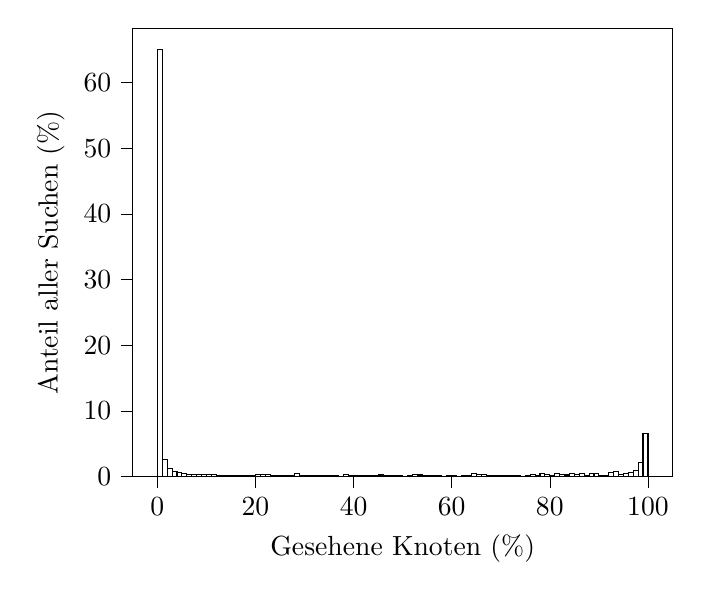
\begin{tikzpicture}

    \begin{axis}[
        tick align=outside,
        tick pos=left,
        x grid style={darkgray176},
        xlabel={Gesehene Knoten (\%)},
        xmin=-5, xmax=105,
        xtick style={color=black},
        xtick={-20,0,20,40,60,80,100,120},
        xticklabels={\ensuremath{-}20,0,20,40,60,80,100,120},
        y grid style={darkgray176},
        ylabel={Anteil aller Suchen (\%)},
        ymin=0, ymax=0.68283477588288,
        ytick style={color=black},
        ytick={0,0.1,0.2,0.3,0.4,0.5,0.6,0.7},
        yticklabels={0,10,20,30,40,50,60,70}
      ]
      \draw[] (axis cs:0,0) rectangle (axis cs:1,0.650318834174171);
      \draw[] (axis cs:1,0) rectangle (axis cs:2,0.0261163959069088);
      \draw[] (axis cs:2,0) rectangle (axis cs:3,0.0121417997603392);
      \draw[] (axis cs:3,0) rectangle (axis cs:4,0.00762458538221844);
      \draw[] (axis cs:4,0) rectangle (axis cs:5,0.00591943697714958);
      \draw[] (axis cs:5,0) rectangle (axis cs:6,0.00413808082213352);
      \draw[] (axis cs:6,0) rectangle (axis cs:7,0.0037684732348896);
      \draw[] (axis cs:7,0) rectangle (axis cs:8,0.00317214759155249);
      \draw[] (axis cs:8,0) rectangle (axis cs:9,0.00266346086065494);
      \draw[] (axis cs:9,0) rectangle (axis cs:10,0.00286922178551252);
      \draw[] (axis cs:10,0) rectangle (axis cs:11,0.00370179145368577);
      \draw[] (axis cs:11,0) rectangle (axis cs:12,0.00250914016701176);
      \draw[] (axis cs:12,0) rectangle (axis cs:13,0.00217954164849032);
      \draw[] (axis cs:13,0) rectangle (axis cs:14,0.0018994781674343);
      \draw[] (axis cs:14,0) rectangle (axis cs:15,0.0015108186427033);
      \draw[] (axis cs:15,0) rectangle (axis cs:16,0.00119455648042266);
      \draw[] (axis cs:16,0) rectangle (axis cs:17,0.00104785656177409);
      \draw[] (axis cs:17,0) rectangle (axis cs:18,0.00181374444874349);
      \draw[] (axis cs:18,0) rectangle (axis cs:19,0.0011621681866949);
      \draw[] (axis cs:19,0) rectangle (axis cs:20,0.000874483930644265);
      \draw[] (axis cs:20,0) rectangle (axis cs:21,0.00245007916080286);
      \draw[] (axis cs:21,0) rectangle (axis cs:22,0.00248246745453029);
      \draw[] (axis cs:22,0) rectangle (axis cs:23,0.00250151939201715);
      \draw[] (axis cs:23,0) rectangle (axis cs:24,0.00151843941769825);
      \draw[] (axis cs:24,0) rectangle (axis cs:25,0.000830664474424814);
      \draw[] (axis cs:25,0) rectangle (axis cs:26,0.00121551361165795);
      \draw[] (axis cs:26,0) rectangle (axis cs:27,0.00128981616785639);
      \draw[] (axis cs:27,0) rectangle (axis cs:28,0.00128219539286178);
      \draw[] (axis cs:28,0) rectangle (axis cs:29,0.0039894757097364);
      \draw[] (axis cs:29,0) rectangle (axis cs:30,0.00172229514880695);
      \draw[] (axis cs:30,0) rectangle (axis cs:31,0.00136792911155248);
      \draw[] (axis cs:31,0) rectangle (axis cs:32,0.00192615087991577);
      \draw[] (axis cs:32,0) rectangle (axis cs:33,0.00115454741170029);
      \draw[] (axis cs:33,0) rectangle (axis cs:34,0.00117740973668445);
      \draw[] (axis cs:34,0) rectangle (axis cs:35,0.00108215004925027);
      \draw[] (axis cs:35,0) rectangle (axis cs:36,0.000988795555565081);
      \draw[] (axis cs:36,0) rectangle (axis cs:37,0.00104023578677936);
      \draw[] (axis cs:37,0) rectangle (axis cs:38,0.000685869749524892);
      \draw[] (axis cs:38,0) rectangle (axis cs:39,0.00248056226078164);
      \draw[] (axis cs:39,0) rectangle (axis cs:40,0.00177373538002135);
      \draw[] (axis cs:40,0) rectangle (axis cs:41,0.00124409151788818);
      \draw[] (axis cs:41,0) rectangle (axis cs:42,0.00176992499252404);
      \draw[] (axis cs:42,0) rectangle (axis cs:43,0.000956407261837544);
      \draw[] (axis cs:43,0) rectangle (axis cs:44,0.00181564964249215);
      \draw[] (axis cs:44,0) rectangle (axis cs:45,0.00151653422394948);
      \draw[] (axis cs:45,0) rectangle (axis cs:46,0.00239292334834229);
      \draw[] (axis cs:46,0) rectangle (axis cs:47,0.00170324321132043);
      \draw[] (axis cs:47,0) rectangle (axis cs:48,0.00103642539928195);
      \draw[] (axis cs:48,0) rectangle (axis cs:49,0.00108215004925039);
      \draw[] (axis cs:49,0) rectangle (axis cs:50,0.00138698104903923);
      \draw[] (axis cs:50,0) rectangle (axis cs:51,0.000621093162069708);
      \draw[] (axis cs:51,0) rectangle (axis cs:52,0.00110882276173196);
      \draw[] (axis cs:52,0) rectangle (axis cs:53,0.00302925806040166);
      \draw[] (axis cs:53,0) rectangle (axis cs:54,0.00227861172342159);
      \draw[] (axis cs:54,0) rectangle (axis cs:55,0.00165561336760311);
      \draw[] (axis cs:55,0) rectangle (axis cs:56,0.00112025392422388);
      \draw[] (axis cs:56,0) rectangle (axis cs:57,0.00205951444232344);
      \draw[] (axis cs:57,0) rectangle (axis cs:58,0.00140793818027474);
      \draw[] (axis cs:58,0) rectangle (axis cs:59,0.000691585330770961);
      \draw[] (axis cs:59,0) rectangle (axis cs:60,0.00104214098052813);
      \draw[] (axis cs:60,0) rectangle (axis cs:61,0.00138698104903912);
      \draw[] (axis cs:61,0) rectangle (axis cs:62,0.000502971149651588);
      \draw[] (axis cs:62,0) rectangle (axis cs:63,0.00190138336118284);
      \draw[] (axis cs:63,0) rectangle (axis cs:64,0.00123266035539626);
      \draw[] (axis cs:64,0) rectangle (axis cs:65,0.00440480794694864);
      \draw[] (axis cs:65,0) rectangle (axis cs:66,0.00320834627277755);
      \draw[] (axis cs:66,0) rectangle (axis cs:67,0.00282159194179543);
      \draw[] (axis cs:67,0) rectangle (axis cs:68,0.00207094560481547);
      \draw[] (axis cs:68,0) rectangle (axis cs:69,0.00175087305503696);
      \draw[] (axis cs:69,0) rectangle (axis cs:70,0.00218144684223898);
      \draw[] (axis cs:70,0) rectangle (axis cs:71,0.00120789283666334);
      \draw[] (axis cs:71,0) rectangle (axis cs:72,0.00121170322416064);
      \draw[] (axis cs:72,0) rectangle (axis cs:73,0.00120598764291446);
      \draw[] (axis cs:73,0) rectangle (axis cs:74,0.00148414593022206);
      \draw[] (axis cs:74,0) rectangle (axis cs:75,0.000682059362027698);
      \draw[] (axis cs:75,0) rectangle (axis cs:76,0.0010040371055543);
      \draw[] (axis cs:76,0) rectangle (axis cs:77,0.00308831906661078);
      \draw[] (axis cs:77,0) rectangle (axis cs:78,0.00205379886107737);
      \draw[] (axis cs:78,0) rectangle (axis cs:79,0.00400090687222843);
      \draw[] (axis cs:79,0) rectangle (axis cs:80,0.00244436357955691);
      \draw[] (axis cs:80,0) rectangle (axis cs:81,0.00208809234855345);
      \draw[] (axis cs:81,0) rectangle (axis cs:82,0.00528119707134167);
      \draw[] (axis cs:82,0) rectangle (axis cs:83,0.00305402557913448);
      \draw[] (axis cs:83,0) rectangle (axis cs:84,0.00230528443590305);
      \draw[] (axis cs:84,0) rectangle (axis cs:85,0.00455341305934576);
      \draw[] (axis cs:85,0) rectangle (axis cs:86,0.00329217479771948);
      \draw[] (axis cs:86,0) rectangle (axis cs:87,0.00422953012207028);
      \draw[] (axis cs:87,0) rectangle (axis cs:88,0.00162322507387547);
      \draw[] (axis cs:88,0) rectangle (axis cs:89,0.00502590110901857);
      \draw[] (axis cs:89,0) rectangle (axis cs:90,0.00425239244705433);
      \draw[] (axis cs:90,0) rectangle (axis cs:91,0.00176039902378056);
      \draw[] (axis cs:91,0) rectangle (axis cs:92,0.00117169415543839);
      \draw[] (axis cs:92,0) rectangle (axis cs:93,0.00560698520236602);
      \draw[] (axis cs:93,0) rectangle (axis cs:94,0.00772746584464701);
      \draw[] (axis cs:94,0) rectangle (axis cs:95,0.00288255814175331);
      \draw[] (axis cs:95,0) rectangle (axis cs:96,0.00501446994652632);
      \draw[] (axis cs:96,0) rectangle (axis cs:97,0.0057098656647947);
      \draw[] (axis cs:97,0) rectangle (axis cs:98,0.00931639743104651);
      \draw[] (axis cs:98,0) rectangle (axis cs:99,0.0207113612419031);
      \draw[] (axis cs:99,0) rectangle (axis cs:100,0.0650433145799436);
    \end{axis}
  \end{tikzpicture}
  \caption{Anteil der pro Suche bei der Erstellung des Contracted-Graph von aegaeis-graph gesehenen Knoten}
  \label{fig:ergebnisse:efficiency_ch_people}
\end{figure}


\subsection{Vertex-to-level Vergeleich}

Wie im \autoref{chapter:peopel} erwähnt, lässt sich durch eine vertex-to-level-Funktion induzierte durchschnittliche Labelgröße vorhersagen, indem für $n$ zufällig ausgewählte Knoten die Labels berechnet und daraus die durchschnittliche Labelgröße bestimmt werden.
Diese Methode wurde verwendet, um verschiedene Funktionen zu testen, deren Ergebnisse in \autoref{table:ergebnisse:vtl_vergleich} aufgeführt sind.

Das verwendete Hitting-Set wurde jeweils über \num{1000000} Pfade gebildet, wobei die Knoten, die nicht im Hitting-Set waren, nach einer weiteren Metrik sortiert wurden.
Verglichen wurden eine Sortierung nach Grad (von klein nach groß), eine zufällige Sortierung sowie die Übernahme der Vertex-to-Level-Funktion, die durch die Graphen-Kontraktion der triangulierten Graphen entstand.
Letztere, in der Tabelle als $\triangle$ als notiert, führte zu überraschend kleinen Labels.

\begin{table}[h!]
  \centering
  \begin{tabular}{l
      S[table-format = 6.0] % random
      S[table-format = 6.0] % random
      S[table-format = 6.0] % random
      S[table-format = 6.0] % random
      S[table-format = 6.0] % random
      S[table-format = 6.0] % random
    }
    \toprule
    Graph              & \multicolumn{3}{c}{Hitting-Set}          & {$\triangle$}     & {Zufällig} & {Grad}   \\ \cline{2-4}
                       & {Zufällig} & {Hits}            & {Grad}  &                   &            &          \\
    \midrule
    aegaeis-visibility & 1747.03    & \bfseries 1420.17 & 1582.00 & 1473.27           & 17811.58   & 7420.85  \\
    medi-visibility    & 2487.06    & 2002.87           & 2422.12 & \bfseries 1930.65 & 18700.13   & 12862.80 \\
    pata-visibility    & 1100.42    & \bfseries 478.80  & 806.95  & 552.90            & 23690.52   & 10174.37 \\
    \bottomrule
  \end{tabular}
  \caption{Vergleich durch level-to-vertex-Funktionen induzierter durschnitliche Labelgröße}
  \label{table:ergebnisse:vtl_vergleich}
\end{table}

\subsection{Hitting-Set über 250M Pfade}

Mit den erzeugten Hub-Graphen wurde ein Hitting-Ste über 250 Millionen Pfade gebildet, die Knoten die nicht enthalten waren, wurden nach der Anzahl ihrerer Hits sortiert, da dies nach \autoref{table:ergebnisse:vtl_vergleich} erfolgsversprechend scheint.
Mit dieser vertex-to-level-Funktion wurde über \num{10000} die Labelgröße predicted.
Für die Sichtbarkeitsgraphen von aegaeis und medi ist die durschnitltiche Label Größe kleiner als der ursprüngliche durschnitliche Knotengrad.

\begin{table}[h!]
  \centering
  \begin{tabular}{ %VERGLEICH
      l % Graph
      r
      S[table-format = 4.1] % average time
    }
    \toprule
    {Graph}            & {Erstellung} & {Label size} \\ \midrule
    aegaeis-graph      & 6h 12m       & 90.8         \\
    aegaeis-visibility & 8h 11m       & 1309.8       \\
    medi-graph         & 4h 47m       & 88.5         \\
    medi-visibility    & 12h 26m      & 1739.4       \\
    pata-graph         &              &              \\
    pata-visibility    & 9h 29m       & 424.1        \\  \bottomrule
  \end{tabular}
  \caption{todo dijkstra vs ch bruteforce vs hl bruteforce}
\end{table}

Mit der enstanden vertex-to-level-Funktion für aegaeis-graph wurde das der \autoref{fig:ergebnisse:efficiency_ch_people} zugrunde liegende Experiment wiederholt, wobei diesmal \num{80.6}\% aller Suchen weniger als 1\% aller Knoten sahen.